\documentclass[12pt]{article}
\usepackage{gensymb}
\usepackage{amsmath}
\usepackage{graphics}
\usepackage{graphicx}
\graphicspath{{storage/self/primary/Download/asgnt9/table}}
\graphicspath{{storage/self/primary/Download/asgnt9/fig}}
\let\vec\mathbf
\usepackage{float}
\providecommand{\brak}[1]{\ensuremath{\left(#1\right)}}
\providecommand{\myvec}[1]{\ensuremath{\begin{pmatrix}#1\end{pmatrix}}}
\providecommand{\norm}[1]{\ensuremath{\lvert|#1\rvert|}}
\begin{document}
\title{\textbf{9.10.6.2}}
\date{}
\maketitle
\textbf{Question :} Two chords $AB$ and $CD$ of lengths $5 cm$ and $11 cm$ respectively of a circle are parallel to each other and are on opposite sides of its centre.If the distance between $AB$ and $CD$ is $6 cm$,find the radius of the circle.

\textbf{Solution :}
\begin{table}[H]
    \centering
       \begin{tabular}{|c|c|c|}
    \hline
    \textbf{Input Parameters} &\textbf{Description} &\textbf{Value} \\
    \hline
     $\vec{O}$& Center(at origin)&$\vec{0}$\\
     \hline
 $r$ & Radius &1\\
 \hline
 $\theta$&-&$100\degree$\\
 \hline
 $\alpha$&-&$165.4\degree$\\
 \hline
 $\beta$&-&$5\degree$\\
 \hline
  \end{tabular}

    \caption{Table of input parameters}
    \label{tab:9.10.6.2.1}
\end{table}
\begin{table}[H]
    \centering
   \begin{tabular}{|c|c|c|}
    \hline
        \textbf{Output Parameters} &\textbf{Description} &\textbf{Value} \\
\hline
          $\vec{Q}$ & Point &$\myvec{\cos{\theta_1}\\\sin{\theta_1}}$\\
          \hline
          $\vec{P}$ & Point &$\myvec{\cos{\theta_2}\\\sin{\theta_2}}$ \\
         \hline
          $\vec{R}$ & Point &$\myvec{\cos{\theta_3}\\sin{\theta_3}}$ \\
         \hline
    \end{tabular}


    \caption{Table of output parameters}
    \label{tab:9.10.6.2.2}
\end{table}
For getting $\theta_1$,
\begin{align}
    AB&=5\\
    2r\cos{\theta_1}&=5\\
    CD&=11\\
    2r\cos{\theta_2}&=11\\
    or,\frac{\cos{\theta_1}}{\cos{\theta_2}}&=\frac{5}{11}\\
    or,\theta_1&=117\degree
    \end{align}
Two chords are parallel and opposite to each other.So,
\begin{align}
   OA^2&=OC^2\\
   OQ^2+CQ^2&=OP^2+PA^2\\
   \brak{OP-OQ}6&=\brak{\frac{11}{2}}^2\brak{\frac{5}{2}}^2\\
   or,OP-OQ&=4\\
   or,OP=5\\
   So,r=OA=OC=5.59cm
    \end{align}
    \begin{figure}[H]                            
\centering
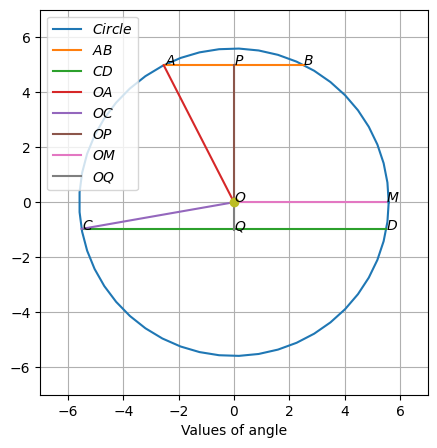
\includegraphics[width=\columnwidth]{fig/9.10.6.2.png}             
\caption{}                              
\label{fig:9.10.6.2}
\end{figure}
\end{document}
